\pagestyle{plain}

\chapter{Análisis de duplicaciones génicas en cepas seleccionadas}\label{apB}

Se puede encontrar el análisis completo para todas las cepas así como una tabla resumen englobando la información contenida en NCBI y los resultados obtenidos en la búsqueda de duplicados en el siguiente enlace:

urla tal cual pascual

\vspace{10mm}
\begin{table}[h]
	\centering
	\captionsetup{width=\linewidth}
	\caption{Tabla resumen de los resultados obtenidos al realizar el proceso de análisis de duplicados con dup\_annot.py en slas cepas seleccionadas.}
	\begin{tabular}{ l || c || c || c || c }
		\hline
		Especie & Cepa & Total proteinas & Grupos & Duplicados \\
		\hline
		\hline
		\multirow{4}{*}{\textit{Klebsiella pneumoniae}} & KpC11 & 5472 & 152 & 270\\
		%\hline
		& ATCC 43816 & 5485 & 124 & 178 \\
		%\hline
		& Beach Ranger & 5040 & 109 & 129 \\
		%\hline
		& KpPF25 & 5222 & 102 & 137 \\
		\hline
		\multirow{4}{*}{\textit{Acinetobacter baumannii}} & ATCC 17961 & 3783 & 122 & 219 \\
		%\hline
		& TP3 & 3571 & 71 & 129 \\
		%\hline
		& TP2 & 3572 & 69 & 124 \\
		%\hline
		& FDAARGOS\_1036 & 3808 & 116 & 205 \\
		\hline
		\multirow{4}{*}{\textit{Pseudomonas aeruginosa}} & DL201330 & 6046 & 116 & 161 \\
		%\hline
		& TJ2014-049 & 6089 & 102 & 158 \\
		%\hline
		& TJ2019-017 & 5904 & 63 & 93 \\
		%\hline
		& TJ2019-022 & 6686 & 191 & 333 \\
		\hline
		\multirow{4}{*}{\textit{Enterobacter cloacae}} & STN0717-73 & 5022 & 92 & 240 \\
		& STN0717-60 & 4522 & 31 & 242 \\
		& RHBSTW-00399 & 5044 & 156 & 242 \\
		& RHBSTW-00490 & 5086 & 157 & 261 \\
		\hline
	\end{tabular}
	\label{table:cepas_result}
\end{table}

\newpage
A continuación se incluyen los gráficos generados con BioCircos para otras cepas de \textit{K. pneumoniae} seleccionadas. El cromosoma de la bacteria (rojo) y sus plásmidos (azul) se representan en un mapa circular que muestra la localización de cada gen duplicado. Las siguientes dos capas muestran los genes en la hebra positiva (rosa) y negativa (turquesa). Las líneas naranja interiores señalan las conexiones entre proteínas pertenecientes al mismo grupo de duplicados. Escala de tamaño en Mb

\vspace{10mm}
\begin{figure}[h]
	\centering
	\captionsetup{width=\linewidth}
	\caption[Gráfica biocircos para la cepa ATCC43816 de \textit{K. pneumoniae}]{Representación gráfica con BioCircos de los genes duplicados en el genoma de la cepa ATCC43816 de \textit{K. pneumoniae}.}
	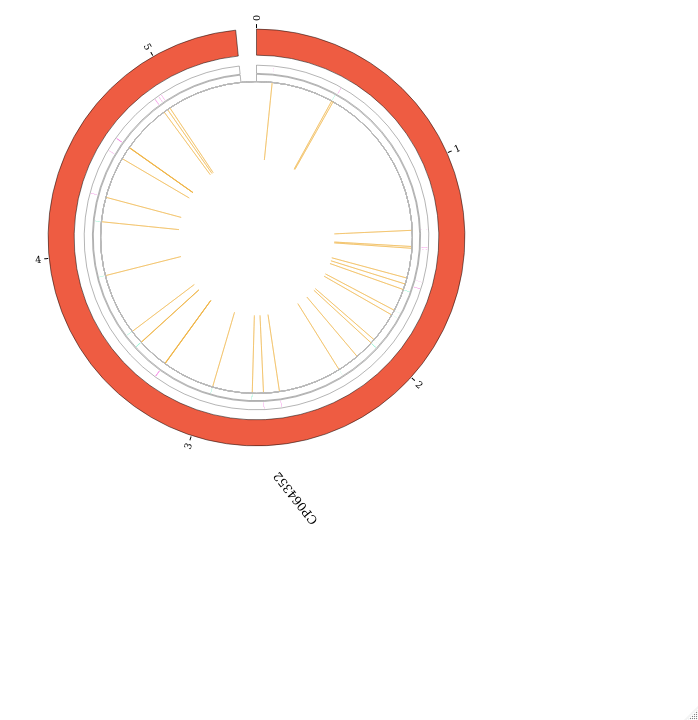
\includegraphics[width=0.8\linewidth]{figs/biocircos_ATCC43816.png}
	\label{fig:bioATCC43816}
\end{figure}

\begin{figure}[h]
	\centering
	\captionsetup{width=\linewidth}
	\caption[Gráfica biocircos para la cepa KpC11 de \textit{K. pneumoniae}]{Representación gráfica con BioCircos de los genes duplicados en el genoma de la cepa KpC11 de \textit{K. pneumoniae}.}
	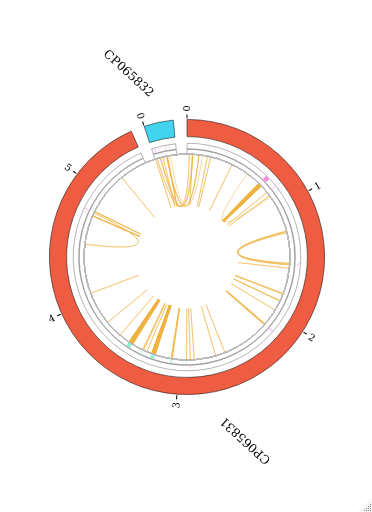
\includegraphics[width=0.8\linewidth]{figs/biocircos_KpC11.png}
	\label{fig:bioKpC11}
\end{figure}

\begin{figure}[h]
	\centering
	\captionsetup{width=\linewidth}
	\caption[Gráfica biocircos para la cepa KpPF25 de \textit{K. pneumoniae}]{Representación gráfica con BioCircos de los genes duplicados en el genoma de la cepa KpPF25 de \textit{K. pneumoniae}.}
	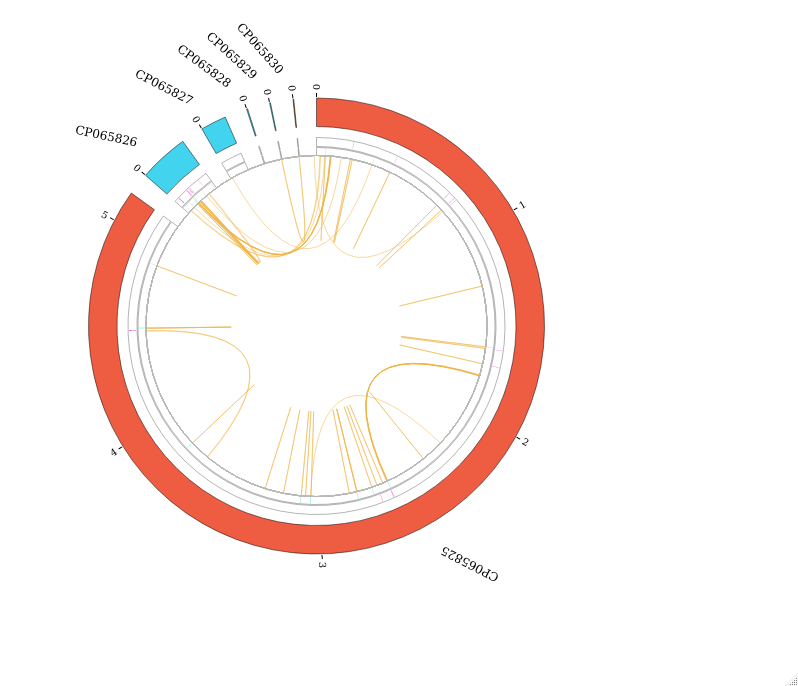
\includegraphics[width=0.8\linewidth]{figs/biocircos_KpPF25.png}
	\label{fig:bioKpPF25}
\end{figure}

